
\documentclass[12pt, a4paper]{exam}
\usepackage{tikz}
\usepackage{textcomp,gensymb}
\usepackage{tfrupee}
\graphicspath{{sdcard/termux/A1/}}

\begin{document}
\begin{center}
    \textbf{ \LaTeX{} Assignment}
\end{center}
\begin{questions}

%Q13 
\question The hour-hand of a clock is 6 cm long . The angle swept by it between 7:20 a.m. and 7:55 a.m. is:

\begin{oneparchoices}
    \choice $(\frac{35}{4})\degree$
    \choice $(\frac{35}{2})\degree$
    \choice 35\degree
    \choice 70\degree
\end{oneparchoices}

%Q18
\question In the given figure, AB $\parallel$ PQ.If AB=6cm,PQ=2 cm and OB=3cm,then the length of OP is:

\begin{figure}[h]
    \centering
    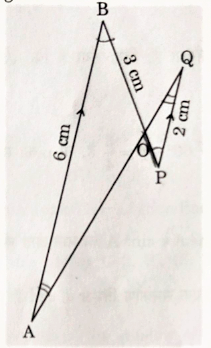
\includegraphics[scale=0.8]{img 1.png}
\end{figure}
\begin{oneparchoices}
    \choice 9cm
    \choice 3cm
    \choice 4cm 
    \choice 1cm
\end{oneparchoices}

%Q24
\question 
\begin{parts}
    \part the length of the shadow of a tower on the plane ground is $\sqrt{3}$ times the height of the tower.Find the angle of elevation of the sun.\\\centerline{\textbf{OR}}

    \part The angle of elevation of the top of a tower from a point on the ground which is 30 m away from the foot of the tower ,is 30\degree.Find the height of the tower.
\end{parts}

%Q29
\question A car has two wipers which do not overlap. Each wiper has a blade of length 21 cm sweeping through an angle of 120\degree. Find the total area cleaned at each sweep of the two blades.

%Q33
\question 
\begin{parts}
    \part As observed from the top of a 75 m high lighthouse from the sea-level,the angles of depression of two ships are 30\degree and 60\degree.If one ship is exactly behind the other on the same side of the lighthouse,find the distance between two ships.\\ (Use $\sqrt{3} = 1.73$) \\\centerline{\textbf{OR}}

    \part From a point on the ground,the angle of elevation of the bottom and top of a transmission tower fixed at the top of 30 m high building are 30\degree and 60\degree,respectively.Find the height of the transmission tower.(Use $\sqrt{3} = 1.73$)
    
\end{parts}

%Q35
\question
\begin{parts}
    \part Sides AB and BC and median AD of a triangle ABC are respectively proportional to sides PQ and QR and median PM of $\Delta$PQR. Show that $\Delta ABC \sim \delta PQR.$ \\\centerline{\textbf{OR}}

    \part Through the mid point M of the CD of a parallelogram ABCD,the line BM is drawn intersecting AC in L and AD(produced) in E.Prove that EL=2BL.
\end{parts}

%Q36
\question
In an annual day function of a school,the organizers wanted to give a cash prize along with a momento to their best students. Each momento is made as shown in  the figure and its base ABCD is shown from the front side. The rate of silver plating is \rupee 20 per $cm^2$.

\begin{figure}[h]
    \centering
    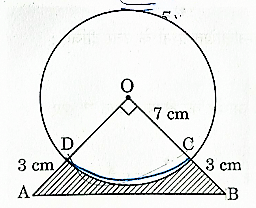
\includegraphics[width=0.5\textwidth]{img2.png}
\end{figure}

Based on the above, answer the following questions:
\begin{parts}
    \part What is the area of the quadrant ODCO?
    \part Find the area of $\Delta$ AOB.
    \part 
    \begin{subparts}
        \subpart What is the total cost of silver plating the shaded part ABCD?\\\centerline{\textbf{OR}}
        \subpart what is the length of arc CD?
    \end{subparts}
    
    
\end{parts}


\end{questions}
\end{document}
